\documentclass[a4paper,UKenglish,cleveref, autoref, thm-restate]{oasics-v2021}
%This is a template for producing OASIcs articles. 
%See oasics-v2021-authors-guidelines.pdf for further information.
%for A4 paper format use option "a4paper", for US-letter use option "letterpaper"
%for british hyphenation rules use option "UKenglish", for american hyphenation rules use option "USenglish"
%for section-numbered lemmas etc., use "numberwithinsect"
%for enabling cleveref support, use "cleveref"
%for enabling autoref support, use "autoref"
%for anonymousing the authors (e.g. for double-blind review), add "anonymous"
%for enabling thm-restate support, use "thm-restate"
%for enabling a two-column layout for the author/affilation part (only applicable for > 6 authors), use "authorcolumns"
%for producing a PDF according the PDF/A standard, add "pdfa"
%
%\pdfoutput=1 %uncomment to ensure pdflatex processing (mandatatory e.g. to submit to arXiv)
%\hideOASIcs %uncomment to remove references to OASIcs series (logo, DOI, ...), e.g. when preparing a pre-final version to be uploaded to arXiv or another public repository
%
%\graphicspath{{./graphics/}}%helpful if your graphic files are in another directory
\usepackage{lmodern}
\usepackage{graphicx}
\usepackage{booktabs}
\usepackage{wrapstuff}
\usepackage{numprint}
\usepackage{wrapfig}
\usepackage{amsfonts}
\usepackage{mathpartir}
\usepackage{tikz}
\usepackage{mystyle}
\usepackage{upquote}
\bibliographystyle{plainurl}% the mandatory bibstyle

\definecolor{blue}{rgb}{0.38, 0.51, 0.71} %glaucous, 97,130,181, #6182B5
\definecolor{darkblue}{RGB}{17, 42, 60} % 112A3C
\definecolor{red}{RGB}{175, 49, 39} % AF3127
\definecolor{orange}{RGB}{217, 156, 55} % D99C37
\definecolor{green}{RGB}{144, 169, 84} % 90A954
\definecolor{palegreen}{RGB}{197, 184, 104} % C5B868
\definecolor{yellow}{RGB}{250, 199, 100} % FAC764
\definecolor{brokenwhite}{RGB}{218, 192, 166} % DAC0A6
\definecolor{brokengrey}{rgb}{0.77, 0.76, 0.82} % {196,194,209}, C4C2D1

\title{Isabelle/Solidity: A Tool  for the Verification of Solidity Smart Contracts} %TODO Please add

%\titlerunning{Dummy short title} %TODO optional, please use if title is longer than one line

\author{Asad {Ahmed}}{University of Exeter, Exeter EX4 4PY, UK \and \url{https://sites.google.com/view/asad-ahmed/home} }{a.ahmed6@exeter.ac.uk}{https://orcid.org/0000-0001-8276-0975}{}%TODO mandatory, please use full name; only 1 author per \author macro; first two parameters are mandatory, other parameters can be empty. Please provide at least the name of the affiliation and the country. The full address is optional. Use additional curly braces to indicate the correct name splitting when the last name consists of multiple name parts.

%\author{Joan R. Public\footnote{Optional footnote, e.g. to mark corresponding author}}{Department of Informatics, Dummy College, [optional: Address], Country}{joanrpublic@dummycollege.org}{[orcid]}{[funding]}
\author{Diego Marmsoler}{University of Exeter, Exeter EX4 4PY, UK}{d.marmsoler@exeter.ac.uk}{https://orcid.org/0000-0003-2859-7673}{}

\authorrunning{J. Open Access and J.\,R. Public} %TODO mandatory. First: Use abbreviated first/middle names. Second (only in severe cases): Use first author plus 'et al.'

\Copyright{Jane Open Access and Joan R. Public} %TODO mandatory, please use full first names. LIPIcs license is "CC-BY";  http://creativecommons.org/licenses/by/3.0/
\begin{CCSXML}
	<ccs2012>
	   <concept>
		   <concept_id>10002978.10002986.10002990</concept_id>
		   <concept_desc>Security and privacy~Logic and verification</concept_desc>
		   <concept_significance>500</concept_significance>
		   </concept>
	 </ccs2012>
\end{CCSXML}

\ccsdesc{Security and privacy~Logic and verification}

\keywords{Program Verification, Smart Contracts, Isabelle, Solidity} %TODO mandatory; please add comma-separated list of keywords

\category{} %optional, e.g. invited paper

\relatedversion{} %optional, e.g. full version hosted on arXiv, HAL, or other respository/website
%\relatedversiondetails[linktext={opt. text shown instead of the URL}, cite=DBLP:books/mk/GrayR93]{Classification (e.g. Full Version, Extended Version, Previous Version}{URL to related version} %linktext and cite are optional

%\supplement{}%optional, e.g. related research data, source code, ... hosted on a repository like zenodo, figshare, GitHub, ...
%\supplementdetails[linktext={opt. text shown instead of the URL}, cite=DBLP:books/mk/GrayR93, subcategory={Description, Subcategory}, swhid={Software Heritage Identifier}]{General Classification (e.g. Software, Dataset, Model, ...)}{URL to related version} %linktext, cite, and subcategory are optional

\funding{This work was supported by the Engineering and Physical Sciences Research Council [grant number EP/X027619/1]}

\acknowledgements{I want to thank \dots}%optional

%\nolinenumbers %uncomment to disable line numbering

%Editor-only macros:: begin (do not touch as author)%%%%%%%%%%%%%%%%%%%%%%%%%%%%%%%%%%
\EventEditors{John Q. Open and Joan R. Access}
\EventNoEds{2}
\EventLongTitle{42nd Conference on Very Important Topics (CVIT 2016)}
\EventShortTitle{CVIT 2016}
\EventAcronym{CVIT}
\EventYear{2016}
\EventDate{December 24--27, 2016}
\EventLocation{Little Whinging, United Kingdom}
\EventLogo{}
\SeriesVolume{42}
\ArticleNo{23}
%%%%%%%%%%%%%%%%%%%%%%%%%%%%%%%%%%%%%%%%%%%%%%%%%%%%%%

\begin{document}

\maketitle

%TODO mandatory: add short abstract of the document
\begin{abstract}
	Recently, formal verification of Solidity smart contracts has drawn a significant attention due to high-risk of financial losses in case of potential vulnerabilities. Most of the formal methods tools are based on the axiomatic approach to ensure bug-free smart contracts. However, the approach does not allow to address the semantic-level abstraction of the programming language thus may lead to miss corner cases. Therefore, in this paper we propose a tool, Isabelle/Solidity, that is based on the design-by-construction approach in Isabelle for Solidity smart contracts. The tool supports formal specification of Solidity smart contracts, invariants, post-conditions and automatic verification of the contracts. A case study, Casino, from the VerifyThis long-term challenge has been presented to showcase the salient features of the proposed tool.
\end{abstract}

\section{Introduction}
\label{sec-intro}

One important innovation which comes with blockchain are so-called \emph{smart contracts}.
These are digital contracts which are automatically executed once certain conditions are met and which are used to automate transactions on the blockchain.
For instance, a payment for an item might be released instantly once the buyer and seller have met all specified parameters for a deal.
Every day, hundreds of thousands of new contracts are deployed~\cite{etherscan:contracts} managing millions of dollars' worth of transactions~\cite{ycharts:transactions}.\looseness-1
%Smart contracts are often used to automate financial transactions and thus they play a central role in the development of \emph{FinTech}, a technological revolution of the financial services sector.
%Therefore, they are of particular importance to the UK, where financial services are one of the largest industries contributing up to 9\% of the total economic output~\cite{Hutton2021}.

Technically, a smart contract is code which is deployed to a blockchain and which can be executed by sending special transactions to it.
Thus, as for every computer program, smart contracts may contain bugs which can be exploited.
However, since smart contracts are often used to automate financial transactions, such exploits may result in huge economic losses.
%For example, in 2016 a vulnerability in an Ethereum smart contract was exploited resulting in a loss of approximately \$60M~\cite{Bahrynovska2017}.
%More recently, hackers had exploited a vulnerability in the DeFi-platform Poly Network to steal \$600M~\cite{BBC2021}.
%As another example, an incorrectly initialised contract was the root cause of the Parity Wallet bug that froze \$280M~\cite{perez.ea:smart:2021}.
In general, it is estimated that since 2019, more than \$5B was stolen due to vulnerabilities in smart contracts~\cite{CipherTrace2021}.
%In the healthcare sector, the impact of such vulnerabilities may be even worse since it may threaten the patients lifes.

The high impact of vulnerabilities in smart contracts together with the fact that once deployed to the blockchain, they cannot be updated or removed easily, makes it important to ``get them right'' before they are deployed.
%Thus, companies have specialised to provide dedicated auditing services in which experts analyse smart contracts for vulnerabilities.
%Unfortunately, however, \highlight{even rigorous security audits cannot guarantee correctness of smart contracts} as shown in a more recent attack in which \$31M was stolen from a smart contract which had received already three security audits throughout the year~\cite{Goodin2021}.

To address this problem we developed Isabelle/Solidity, a framework for the verification of Solidity smart contracts.
The main aim of this paper is to introduce the Isabelle/Solidity tool for the verification of Solidity Smart Contracts.
To this end its contribution is two-fold:
\begin{itemize}
	\item We describe the architecture of Isabelle/Solidity
	\item We demonstrate it by verifying the Casino Contract from the long term verification challenge.
\end{itemize}

\section{Overview}
\label{sec-overview}

\autoref{fig:approach} depicts an overview of our approach to verify Solidity smart contract.
\begin{figure}[!h]
    \centering
    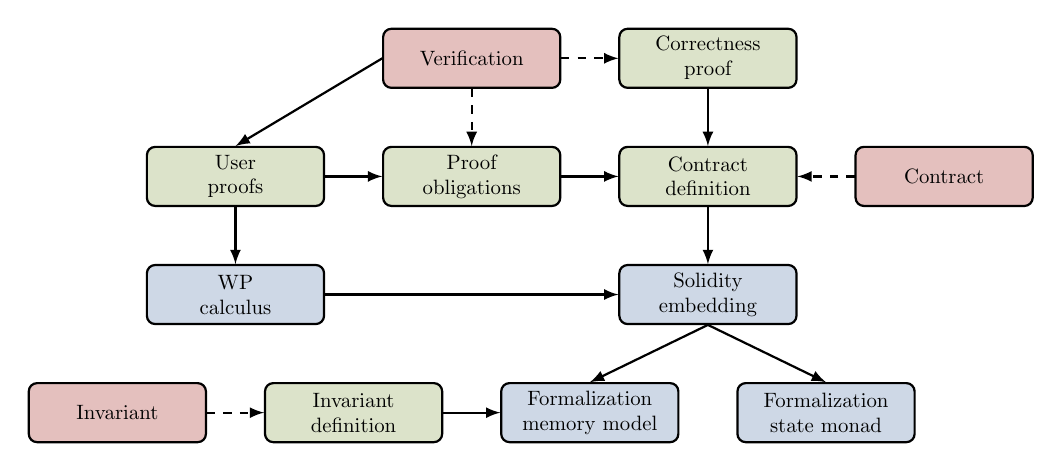
\begin{tikzpicture}[%
        thick,scale=0.75, every node/.style={scale=0.75},
        basic/.style ={rounded corners=3pt, draw, minimum width=3cm, minimum height=1cm, align=center},
        theory/.style={basic, fill=blue!95!black!30},
        temp/.style={basic, fill=green!95!black!30},
        feature/.style={basic, fill=red!95!black!30},
        dep/.style={-latex},
        gen/.style={-latex,dashed}
        ]
        \node[feature] (ver) at (0,0) {Verification};
        \node[temp] (obl) at (0,-2) {Proof \\ obligations};
        \node[temp] (usr) at (-4,-2) {User \\ proofs};
        \node[temp] (cor) at (4,0) {Correctness \\ proof};
        \node[temp] (cnt) at (4,-2) {Contract \\ definition};
        \node[feature] (spc) at (8,-2) {Contract};
        \node[theory] (wpc) at (-4,-4) {WP \\ calculus};
        \node[theory] (lan) at (4,-4) {Solidity \\ embedding};
        \node[feature] (isc) at (-6,-6) {Invariant};
        \node[temp] (idf) at (-2,-6) {Invariant \\ definition};
        \node[theory] (fmm) at (2,-6) {Formalization \\ memory model};
        \node[theory] (fsm) at (6,-6) {Formalization \\ state monad};
        \draw[dep] (ver.west) -- (usr.north);
        \draw[gen] (ver.south) -- (obl.north);
        \draw[gen] (ver.east) -- (cor.west);
        \draw[dep] (cor.south) -- (cnt.north);
        \draw[gen] (spc.west) -- (cnt.east);
        \draw[dep] (usr.south) -- (wpc.north);
        \draw[dep] (usr.east) -- (obl.west);
        \draw[dep] (obl.east) -- (cnt.west);
        \draw[dep] (cnt.south) -- (lan.north);
        \draw[dep] (wpc.east) -- (lan.west);
        \draw[dep] (lan.south) -- (fsm.north);
        \draw[dep] (lan.south) -- (fmm.north);
        \draw[dep] (idf.east) -- (fmm.west);
        \draw[gen] (isc.east) -- (idf.west);
    \end{tikzpicture}
    \caption{Isabelle/Solidity: Overview of theories (blue), commands (red), and generated artefacts (green). \label{fig:approach}}
\end{figure}
Our framework is based on four Isabelle theories which are represented by the {\color{blue}blue rectangles}:
\begin{description}
    \item[Formalization state monad]
    In our framework we model Solidity programs as functions which manipulate states.
    Such functions are usually described in terms of state monads~\cite{Wadler1993} and this theory contains our formalization of it based on \cite{Cock2008}.
    \item[Formalization memory model]
    Solidity has a quite particular memory model with different types of stores which support different types of data structures.
    This theory contains our formalization of the Solidity memory model as a deep embedding.
    It also defines the notion of a Solidity state as a collection of different stores.
    \item[Solidity embedding]
    A Solidity statement is defined as a particular state monad manipulating a Solidity state.
    This theory contains definitions for all our Solidity statements.
    \item[WP calculus]
    To support a user in the verification of properties for our Solidity programms we provide a weakest precondition calculus~\cite{Dijkstra1975} for our Solidity statements.
    This theory formalizes the calculus.
\end{description}

Our framework extends Isabelle by means of three new definitional commands represented by the {\color{red}red rectangles} in \autoref{fig:approach}.
Each of the commands generates lower level definitions and theorems for Isabelle/HOL which are represented as {\color{green}green rectangles}.
\begin{description}
    \item[Contract]
    This command allows a user to specify a new contract.
    It requires a user to specify a list of member variables, a constructor, and a list of methods.
    For each method the user can specify a list of parameters as well as a method body.
    The body is provided as a state monad using the monads defined in the corresponding Isabelle theory.
    The command then generates definitions for the \emph{contracts methods}.
    To this end each method is mapped to a corresponding partial function definition~\cite{Krauss2010}.
    \item[Invariant]
    This command support a user in the specification of an invariant for the contract.
    An invariant is specified as a HOL formula over the store and balance of the contract.
    The command then integrates the typing information of member variables to generates a corresponding \emph{invariant definition}.
    \item[Verification]
    This command triggers the verification of a contract.
    It requires a user to provide an invariant as well as postconditions for the methods.
    Then it presents the user with a list of \emph{proof obligations} for each of the contracts methods.
    The users must then discharge these proof obligations by providing a corresponding \emph{proof}.
    To this end they can use the WP calculus provided by our framework.
    After discharging these obligations our framework then proves an overall \emph{correctness theorem} which guarantees that the invariant as well as postconditions are not violated.
\end{description}

\section{Case Study}
We use  a case study, Casino, from VerifyThis long-term challenge. 
%
Casino is a betting game based on guessing the outcome of coin-tossing and is implemented using Solidity syntax (see Appendix \ref{sec:app1}).
%
Anytime, the game is characterized by three states, i.e., \texttt{IDLE}, \texttt{GAME\_AVAILABLE} and \texttt{BET\_PLACED}.
%
Initially, game is in \texttt{IDLE} state.
%
The game has been implemented using following functions in Solidity:
%
\begin{itemize}
\item Only operator can create a game by calling \texttt{creatGame} function which changes the state to \texttt{GAME\_AVAILABLE},  and also requires a secret number from the player to ensure unbiased and verifiable bet.
%
\item Once in \texttt{GAME\_AVAILABLE} state, a player can place a bet by invoking \texttt{placeBet} fucntion. 
%
This function saves the bet (\texttt{HEAD} or \texttt{TAIL}), amount of the bet and changes the state to \texttt{BET\_PLACED}.
\item Now, operator can decide the bet anytime by calling \texttt{decideBet} function by providing secret number generated when game was created.
%
It allows the function to verify the bet and also decide the outcome of the coin tossing (\texttt{HEAD} or \texttt{TAIL}).
%
If player wins then double the amount of the bet is transferred to the player else amount equal to the bet is transferred to the operator.
%
It also changes the state of the game to \texttt{IDLE} state.
\item Operator may add money to the bet, at anytime,  using \texttt{addToPot} but can only remove if game is in not in \texttt{BET\_PLACED} state by calling \texttt{decideBet}.
\end{itemize}
%
%%THIS CAN MOVE UP IN THE INTRODUCTION
The Casino smart contract is selected for two accounts: One, it has been implemented using sophisticated and advanced features of Solidity syntax including data types, global and local variables, functions, modifiers and precondition specifiers. 
%
Thus, requires to develop powerful equivalent syntax support in the proposed tool to embed the program logic. Two, from verification aspect, Casino has been employed as a case study in literature and hence allows to compare and report the result to gauge the performance of the proposed tool, comparatively.
%
%
\section{Specification}
In this section, we present a Solidity equivalent specification of smart contracts in Isabelle/Solidity. 
%
We primarily focused on specifications of state or local variables, data types, functions, modifiers, precondition specifiers and statements in Isabelle/Solidity.
%\vspace{-1cm}
\paragraph*{Storage Variables}
%
%
In Listing \ref{fig:isadt}, Casino smart contract is defined using Isabelle/Solidity command \texttt{\color{isacom}contract} followed by \emph{name} and list of storage variables.
%
The tool, also,  allows data-type annotations to specify the types of variables (Listing \ref{fig:isadt}).
\begin{code}{label={fig:isadt}}{isabelle}{Isabelle/Solidity data types for Casino}
contract Casino
  for state: "SType.TValue TSint"
  and operator: "SType.TValue TAddress"
  and player: "SType.TValue TAddress"
  and pot: "SType.TValue TSint"
  and hashedNumber: "SType.TValue TBytes"
  and bet: "SType.TValue TSint"
  and guess: "SType.TValue TSint"

constructor payable
where
  "skip"
\end{code}
%
\paragraph*{Methods}
%
%
A function, \texttt{decideBet}, in Listing \ref{fig:isamethod} showcases Isabelle/Solidity features to specify Solidity functions.
%
The keyword \texttt{\color{isargreen}emethod} defines \texttt{decideBet} which has a \texttt{\color{isargreen}payable}  modifier. 
%
A memory (local) variable, \texttt{secretNumber}, of  integer type is declared using keyword  \texttt{\color{isargreen}param}.
%
Isabelle/Solidity allows to specify the body of the function using \texttt{\color{isargreen}where} \texttt{"do \{\dots\}",} structure.
%
%
\begin{code}{label={fig:isamethod}}{isabelle}{Isabelle/Solidity method for Casino}
emethod decideBet payable
  param secretNumber: "SType.TValue TSint"
where
  "do {
    byOperator;
    inState (valtype.Sint 2);
    $\langle$assert$\rangle$ ((hashedNumber $\sim\textsubscript{s}$ []) $\langle$=$\rangle$ ($\langle$keccak256$\rangle$ (secretNumber $\sim$ [])));
    decl TSint secret;
    secret [] ::= IF ((secretNumber $\sim$ []) $\langle\%\rangle$ $\langle$sint$\rangle$ 2) $\langle$=$\rangle$( $\langle$sint$\rangle$ 0) 
    					THEN $\langle$sint$\rangle$ 0 ELSE $\langle$sint$\rangle$ 1;
    IF (secret $\sim$ []) $\langle$=$\rangle$(guess $\sim\textsubscript{s}$ []) THEN
      do {
        decl TSint bet_old;
        bet_old [] ::= bet $\sim\textsubscript{s}$ [];
        bet [] ::=$\textsubscript{s}$ $\langle$sint$\rangle$ 0;
        pot [] ::=$\textsubscript{s}$ ((pot $\sim\textsubscript{s}$ []) $\langle$-$\rangle$ (bet_old $\sim$ []));
        $\langle$transfer$\rangle$ (player $\sim\textsubscript{s}$ []) ((bet $\sim\textsubscript{s}$ []) $\langle$*$\rangle$ ($\langle$sint$\rangle$ 2))
      }
     ELSE
      do {
        pot [] ::=$\textsubscript{s}$ pot $\sim\textsubscript{s}$ [] $\langle$+$\rangle$ bet $\sim\textsubscript{s}$ [];
        bet [] ::=$\textsubscript{s}$ $\langle$sint$\rangle$ 0
      };
     state [] ::=$\textsubscript{s}$ $\langle$sint$\rangle$ 0
  }",
\end{code}
%
Lines 5-7, implement preconditions for Casino, i.e., only operator can call the function, game should be in \texttt{IDLE} state and \texttt{secretNumber} should be equal to the \texttt{hashedNumber}. 
%
For this purpose, Isabelle/Solidity employs \texttt{\color{isarblue}{assert}} which models the Solidity \texttt{\color{blue}{require}} command. 
%
That is, if preconditions are not met then \texttt{\color{isarblue}{assert}} throws an exception.
%
%
%
%
%

%
Isabelle/Solidity also supports Solidity statements such as control structures and assignment operators. 
%
For example, in Line 9, \texttt{\color{isarblue}{IF}}\dots \texttt{\color{isarblue}{THEN}}\dots \texttt{\color{isarblue}{ELSE}} reveals \texttt{HEAD} or \texttt{TAIL} by taking the  modulus (\texttt{$\langle\%\rangle$})of \texttt{secretNumber}. 
%
For assignment operators, Isabelle/Solidity employs storage (::=) and stack (::=$\textsubscript{s}$) assignment operators along with search operators ($\sim$ and $\sim\textsubscript{s}$ ) for respective stores. 
%

%
%Next, 
%%
%in Line 10 (of Listing \ref{fig:isamethod}), \texttt{transfer\_monad} transfers (special function) an amount  equal to the bet is transferred to the operator account.
%

%
%
\section{Verification}
%
%
%
Isabelle/Solidity facilitates invariance specification using \texttt{\color{isarblue}invariant} command over the contract balance and storage.
%
This command requires a user to provide the name of the invariant, followed by the invariant as predicates formulated over the contract's store and balance. The command then generates introduction and elimination rules which can be invoked for automated verification of the invariants.
%
\begin{Example}{Invariant}{invariant}
	Assume that we want to verify that when game is in  \texttt{BET\_PLACED} state, contract's internal balance satisfies:
	\begin{equation}
		pot\_balance(s, b)=b \ge s(\STR{pot}) + s(\STR{bet})  \quad\wedge\quad s(\STR{bet}) \leq s(\STR{pot})
	\end{equation}\label{eq:inv}
	and if not in \texttt{BET\_PLACED}, then 
\begin{equation}
		pot\_balance(s, b)=b \ge pot 
	\end{equation}\label{eq:inv1}
Above invariant ensures payout safety for players by explicitly placing upper bound on the contract balance w.r.t the amount of bet and pot  in  \texttt{BET\_PLACED} state and otherwise.
%

%
The corresponding specification in Isabelle/Solidity is given in Listing \ref{def:inv}:
\begin{code}{label={def:inv}}{isabelle}{Invariant in Isabelle/Solidity}
invariant pot_balance sb where
    "(fst sb STR ''state'' = sdata.Value (Sint 2)
      $\longrightarrow$ snd sb $\geq$ unat (valtype.sint (sdata.vt (fst sb STR ''pot''))) 
		+ unat (valtype.sint (sdata.vt (fst sb STR ''bet'')))
        $\wedge$ valtype.sint (sdata.vt (fst sb STR ''bet'')) $\leq$ 
		valtype.sint (sdata.vt (fst sb STR ''pot''))) $\wedge$
    (fst sb STR ''state'' $\neq$ sdata.Value (Sint 2)
    $\longrightarrow$  snd sb $\geq$ unat (valtype.sint (sdata.vt (fst sb STR ''pot''))))"
  for "casino"
\end{code}
\end{Example}
%

%
To formally verify the invariant, Isabelle/Solidity allows to specify the verification of invariants using \texttt{\color{isarblue}verificaiton} command. 
%
It accepts the name of the invariant, invariant and postconditions on the constructor and methods to generate proof obligations. 
%
For example, in Listing \ref{def:ver}, \texttt{creatGame\_post} is a postcondition that ensures that state of the game will be \texttt{creatGame} after the execution of \texttt{creatGame} fucntion.
%
In order to automate the verification task, the tool has weakest precondition calculus based verification condition generator to discharge the proof obligations.

\begin{code}{label={def:ver}}{isabelle}{Verification in Isabelle/Solidity}
verification pot_balance:
   pot_balance
  "K (K (K True))"
  "createGame" "createGame_post" and
  "placeBet" "placeBet_post" and
  "decideBet" "decideBet_post" and
  "addToPot" "K (K (K True))" and
  "removeFromPot" "K (K (K (K True)))"
  for "casino"
\end{code}
%\vskip
%\paragraph*{Discussions}
Verification of the Casino smart contract using Isabelle/Solidity resulted in the exploration of a major vulnerability, i.e., Reenetrancy.
%
While verifying the invariant in Example \autoref{ex:invariant},  it was not possible to verify unless changing the order of the Line 32 and 33 (see Appendix \ref{sec:app1}) which enabled the completion of the verification task. 
%
It is due to possibility of calling the function \texttt{decideBet} without setting \texttt{bet}=\texttt{0} which may lead to unintended behaviour.  
%

\section{Related Work}
%
Considering the mission-critical nature of the smart contracts in blockchain technology, various formal methods techniques, such as Model Checking, theorem proving and SMT solvers, have been employed to formally specify and verify Solidity smart contracts. 
%
Solidifier \cite{antonino2020formalising}, VeriSol\footnote{\url{https://github.com/Microsoft/verisol}} and solc-verify \cite{hajdu2020solc} translates a given smart contract into equivalent Boogie script, an intermediate verification language, which is then employed for formal verification using bounded model checking and SMT solvers.
%
Model checking is a push-button automatic  formal methods technique, however, has limited expressiveness due to finite-state machine modelling and is prone to state-space explosion.
%

%
Theorem proving is highly-expressive formal methods technique and has also been employed to formally specify and verify Solidity smart contracts. 
%
SolidiKeY \cite{ahrendt2020functional} accomplishes the task of verification using KeY theorem prover for a given smart contract specified as a dynamic logic (DL) formula. 
%
An intermediary low-level specification language, \texttt{SOLI} \cite{ribeiro2020formal}, allows to formally specify and verify smart contracts in Isabelle/HOL (\textcolor{red}{I doubt if it is axiomatic approach for Solidity smart contracts, need your comments}). 
%Jackob  has proposed an interpreter in Coq theorem prover for Solidity using big-step semantic approach. 
%
%These efforts allow to formally specify and verify the Solidity smart contracts deductively using native proof theories in corresponding theorem provers. 
%
The above-mentioned research work  is based on axiomatic approach, thus, limits  verification capabilities of Solidity smart contracts. 
%
To overcome this issue, correct by construction approach has also been employed to formally specify and verify smart contracts.
%
Particularly, deep \cite{marmsoler2022isabelle} and shallow embedding \cite{marmsoler2024secure} of Solidity in Isabelle/HOL facilitate formal specification and verification of Solidity smart contracts.
%
Also we follow a definitional approach meaning that we generate lower level definitions from higher level domain constructs which ensures consistency by construction.
 %Particularly, deep embedding of Solidity statements as a datatype in Isabelle/HOL \cite{marmsoler2022isabelle} facilitates deductive reasoning about the language itself which in turn allows to formally specify and verify complex properties of Solidity smart contracts. 
%
%
%
%On the other hand, Isabelle/Solidity \cite{marmsoler2024secure} leverages upon the shallow embedding of Solidity in Isabelle/HOL in order to reduce the signification effort for verifying smart contracts with deep embedding approach.
%

%
 Isabelle/Solidity tool, proposed in this paper, is based on the shallow embedding approach \cite{marmsoler2024secure}. 
% 
 Although, deep embedding furnishes deductive reasoning about the Solidity language itself but results in a significant effort to develop full support for the purpose.  
%
On the other hand, shallow embedding approach  offers  
%
%Also we follow a definitional approach meaning that we generate lower level definitions from higher level domain constructs which ensures consistency by construction.
%

\section{Conclusion}
%%
%% Bibliography
%%
%
In this paper, we present Isabelle/Solidity tool for the formal specification and verification of Solidity smart contracts. 
%
The tool facilitates Solidity data-types, functions, modifiers, statements, expressions and post/pre-condition specifiers in Isabelle/HOL.
%
%
The formal specification relies upon the underlying shallow embedding of Solidity expressions and statements as state-monads and storage models for different types of stores in Solidity.
%
For the verification purpose, tool supports invariant specification for the contract that in turn is supported by verification condition generator to automate the verification process.
%
Finally, we evaluated the approach by means of the Casino case study.
%
The use of the Isabelle/Solidity resulted in the exploration of re-entrancy vulnerability in the original version of Casino smart contract.
%
However, there are few  challenges in order to  fully cover the advanced features of Solidity. 
%

%
In this regard, inheritance is one of the most notable Solidity feature which can be introduced in the proposed tool for verifying interesting properties of the smart contracts.
%
Moreover, from the verification point-of-view, automation can be further improved by providing specialized rules w.r.t the context of the smart contracts.


%
%% Please use bibtex, 
%\nocite{*}
\bibliography{oasics-v2021-sample-article}

\appendix

\section{Casino: Solidity Smart Contract}\label{sec:app1}


\begin{code}{label={fig:casino}}{solidity}{Solidity source code for the Casino}
	contract Casino {
		enum Coin { HEADS, TAILS } ;
		enum State { IDLE, GAME_AVAILABLE,  BET_PLACED }
		State private state; 
		address public operator, player;
		uint public pot;
		bytes32 public hashedNumber;
		uint public bet;
		Coin guess;

		function createGame(bytes32 hashNum) 
			public byOperator, inState(IDLE) { 
			hashedNumber = hashNum; 
			state = GAME_AVAILABLE;
		}

		function placeBet(Coin _guess) public payable inState(GAME_AVAILABLE) {
			require (msg.sender != operator);
			require (msg.value <= pot);
			state = BET_PLACED; 
			player = msg.sender; 
			bet = msg.value; 
			guess = _guess; 
		}

 		function decideBet(uint secretNumber) 
		public byOperator, inState(BET_PLACED) { 
			require (hashedNumber == keccak256(secretNumber)); 
			Coin secret = (secretNumber % 2 == 0)? HEADS : TAILS;
			if (secret == guess) {
				pot = pot - bet;  
				player.transfer(bet*2);  
				bet = 0;} 
			else {
				pot = pot + bet; 
				bet = 0;
				}
			state = IDLE;}
		function addToPot() public payable byOperator { pot = pot + msg.value;}

		function removeFromPot(uint amount) public byOperator, noActiveBet { 
			operator.transfer(amount);  
			pot = pot - amount;}
		}
\end{code}


%\cref{testenv-proposition} and \autoref{testenv-proposition} ...
%
%\section{Theorem-like environments}\label{sec:theorem-environments}
%
%List of different predefined enumeration styles:
%
%\begin{theorem}\label{testenv-theorem}
%Fusce eu leo nisi. Cras eget orci neque, eleifend dapibus felis. Duis et leo dui. Nam vulputate, velit et laoreet porttitor, quam arcu facilisis dui, sed malesuada risus massa sit amet neque.
%\end{theorem}
%
%\begin{lemma}\label{testenv-lemma}
%Fusce eu leo nisi. Cras eget orci neque, eleifend dapibus felis. Duis et leo dui. Nam vulputate, velit et laoreet porttitor, quam arcu facilisis dui, sed malesuada risus massa sit amet neque.
%\end{lemma}
%
%\begin{corollary}\label{testenv-corollary}
%Fusce eu leo nisi. Cras eget orci neque, eleifend dapibus felis. Duis et leo dui. Nam vulputate, velit et laoreet porttitor, quam arcu facilisis dui, sed malesuada risus massa sit amet neque.
%\end{corollary}
%
%\begin{proposition}\label{testenv-proposition}
%Fusce eu leo nisi. Cras eget orci neque, eleifend dapibus felis. Duis et leo dui. Nam vulputate, velit et laoreet porttitor, quam arcu facilisis dui, sed malesuada risus massa sit amet neque.
%\end{proposition}
%
%\begin{conjecture}\label{testenv-conjecture}
%Fusce eu leo nisi. Cras eget orci neque, eleifend dapibus felis. Duis et leo dui. Nam vulputate, velit et laoreet porttitor, quam arcu facilisis dui, sed malesuada risus massa sit amet neque.
%\end{conjecture}
%
%\begin{observation}\label{testenv-observation}
%Fusce eu leo nisi. Cras eget orci neque, eleifend dapibus felis. Duis et leo dui. Nam vulputate, velit et laoreet porttitor, quam arcu facilisis dui, sed malesuada risus massa sit amet neque.
%\end{observation}
%
%\begin{exercise}\label{testenv-exercise}
%Fusce eu leo nisi. Cras eget orci neque, eleifend dapibus felis. Duis et leo dui. Nam vulputate, velit et laoreet porttitor, quam arcu facilisis dui, sed malesuada risus massa sit amet neque.
%\end{exercise}
%
%\begin{definition}\label{testenv-definition}
%Fusce eu leo nisi. Cras eget orci neque, eleifend dapibus felis. Duis et leo dui. Nam vulputate, velit et laoreet porttitor, quam arcu facilisis dui, sed malesuada risus massa sit amet neque.
%\end{definition}
%
%\begin{example}\label{testenv-example}
%Fusce eu leo nisi. Cras eget orci neque, eleifend dapibus felis. Duis et leo dui. Nam vulputate, velit et laoreet porttitor, quam arcu facilisis dui, sed malesuada risus massa sit amet neque.
%\end{example}
%
%\begin{note}\label{testenv-note}
%Fusce eu leo nisi. Cras eget orci neque, eleifend dapibus felis. Duis et leo dui. Nam vulputate, velit et laoreet porttitor, quam arcu facilisis dui, sed malesuada risus massa sit amet neque.
%\end{note}
%
%\begin{note*}
%Fusce eu leo nisi. Cras eget orci neque, eleifend dapibus felis. Duis et leo dui. Nam vulputate, velit et laoreet porttitor, quam arcu facilisis dui, sed malesuada risus massa sit amet neque.
%\end{note*}
%
%\begin{remark}\label{testenv-remark}
%Fusce eu leo nisi. Cras eget orci neque, eleifend dapibus felis. Duis et leo dui. Nam vulputate, velit et laoreet porttitor, quam arcu facilisis dui, sed malesuada risus massa sit amet neque.
%\end{remark}
%
%\begin{remark*}
%Fusce eu leo nisi. Cras eget orci neque, eleifend dapibus felis. Duis et leo dui. Nam vulputate, velit et laoreet porttitor, quam arcu facilisis dui, sed malesuada risus massa sit amet neque.
%\end{remark*}
%
%\begin{claim}\label{testenv-claim}
%Fusce eu leo nisi. Cras eget orci neque, eleifend dapibus felis. Duis et leo dui. Nam vulputate, velit et laoreet porttitor, quam arcu facilisis dui, sed malesuada risus massa sit amet neque.
%\end{claim}
%
%\begin{claim*}\label{testenv-claim2}
%Fusce eu leo nisi. Cras eget orci neque, eleifend dapibus felis. Duis et leo dui. Nam vulputate, velit et laoreet porttitor, quam arcu facilisis dui, sed malesuada risus massa sit amet neque.
%\end{claim*}
%
%\begin{proof}
%Fusce eu leo nisi. Cras eget orci neque, eleifend dapibus felis. Duis et leo dui. Nam vulputate, velit et laoreet porttitor, quam arcu facilisis dui, sed malesuada risus massa sit amet neque.
%\end{proof}
%
%\begin{claimproof}
%Fusce eu leo nisi. Cras eget orci neque, eleifend dapibus felis. Duis et leo dui. Nam vulputate, velit et laoreet porttitor, quam arcu facilisis dui, sed malesuada risus massa sit amet neque.
%\end{claimproof}

\end{document}
